% !TEX root = ../main.tex

% = = = = = = = = = = = = = = = = = = = = = = = = = = = = = = = = = = = = = = = = = =

\section{Introductory Remarks}

Capitalization, infrastructure, and regulation make new deployments of financial technology challenging. Blockchain systems like Ethereum radically reduce the barrier-to-entry by allowing anyone to deploy any solution, provided it can operate autonomously as software. The key promise of code running on Ethereum is that the code will execute exactly as it is written, and the code that is written can never be changed. Ethereum cannot maintain this promise unconditionally but its assumptions---that certain cryptographic primitives are secure, and that well-intentioned participants outweigh malicious ones---provide a realistic level of assurance. 

The immutability of a smart contract's code is related to trust. If Alice can validate the code of a contract, she can trust her money to it and not be surprised by its behaviour. Unfortunately, disguising malicious behaviour in innocuous-looking code is possible, and many blockchain users have been victims of such contracts (`rug pulls'). On the other hand, if the smart contract is long-standing with lots of attention, and perhaps assessments from third-party professional auditors, the immutability of the code can add confidence. 

Consider the case where a security vulnerability in the code of a smart contract is discovered. The flip-side of immutability is that it prevents software updates. Less urgently, some software projects may want to roll out new features, which is also blocked by immutability. There is an intense debate about whether this is a positive or negative, with many claiming that `upgradability is a bug.' We do not take a position on this debate. We note that upgradability is happening and we seek to study what is already being done and what is possible. 

Is there a way to deploy upgradeable smart contracts if all smart contracts are (practically speaking) immutable? Consider a two simple ideas. The first is to deploy the upgraded smart contract at a new address. One main drawback to this is that all software and websites need to update their addresses. A second simple idea is to use a proxy contract (call it P) that stores the address of the `real' contract (call it A). Users consider the system to deployed at P (and might not even be aware it is proxy). When a function is called on P, it is forwarded to A. When an upgrade is deployed to a new address (call it B), the address in P is changed from A to B. This solution also has drawbacks. For example, if the proxy contract hardcodes the list of functions that might be called on A, new functions cannot be added to B. Another issues is that the data (contract state) is stored in A. For most applications, a snapshot of A's state will need to be copied to B without creating race conditions. Mitigating these issues leads to more elaborate solutions like splitting contract logic and state between different contracts, utilizing Ethereum-specific tricks (fallback functions to capture unexpected function names), and trying to reduce the inefficiencies of using a cluster of contracts.

\paragraph{Contributions.} 

\textblue{Finalize this text later.} %In the following sections we classify different ways of upgradeability on Ethereum blockchain, and describe pros and cons of each approach. Then we evaluate the upgradeability methods and compare them with each other. We conducted a measurement study in the most favorable upgrade pattern in Ethereum blockchain and give a dataset of them. Also we will talk about possible agents that is responsible for the changes on the Dapps. In the last part we will talk about some problems we are facing in the upgrade process and the ways that we can handle them.

% = = = = = = = = = = = = = = = = = = = = = = = = = = = = = = = = = = = = = = = = = =

\section{Background and Related Work}

\begin{figure}[t]
  \centering
      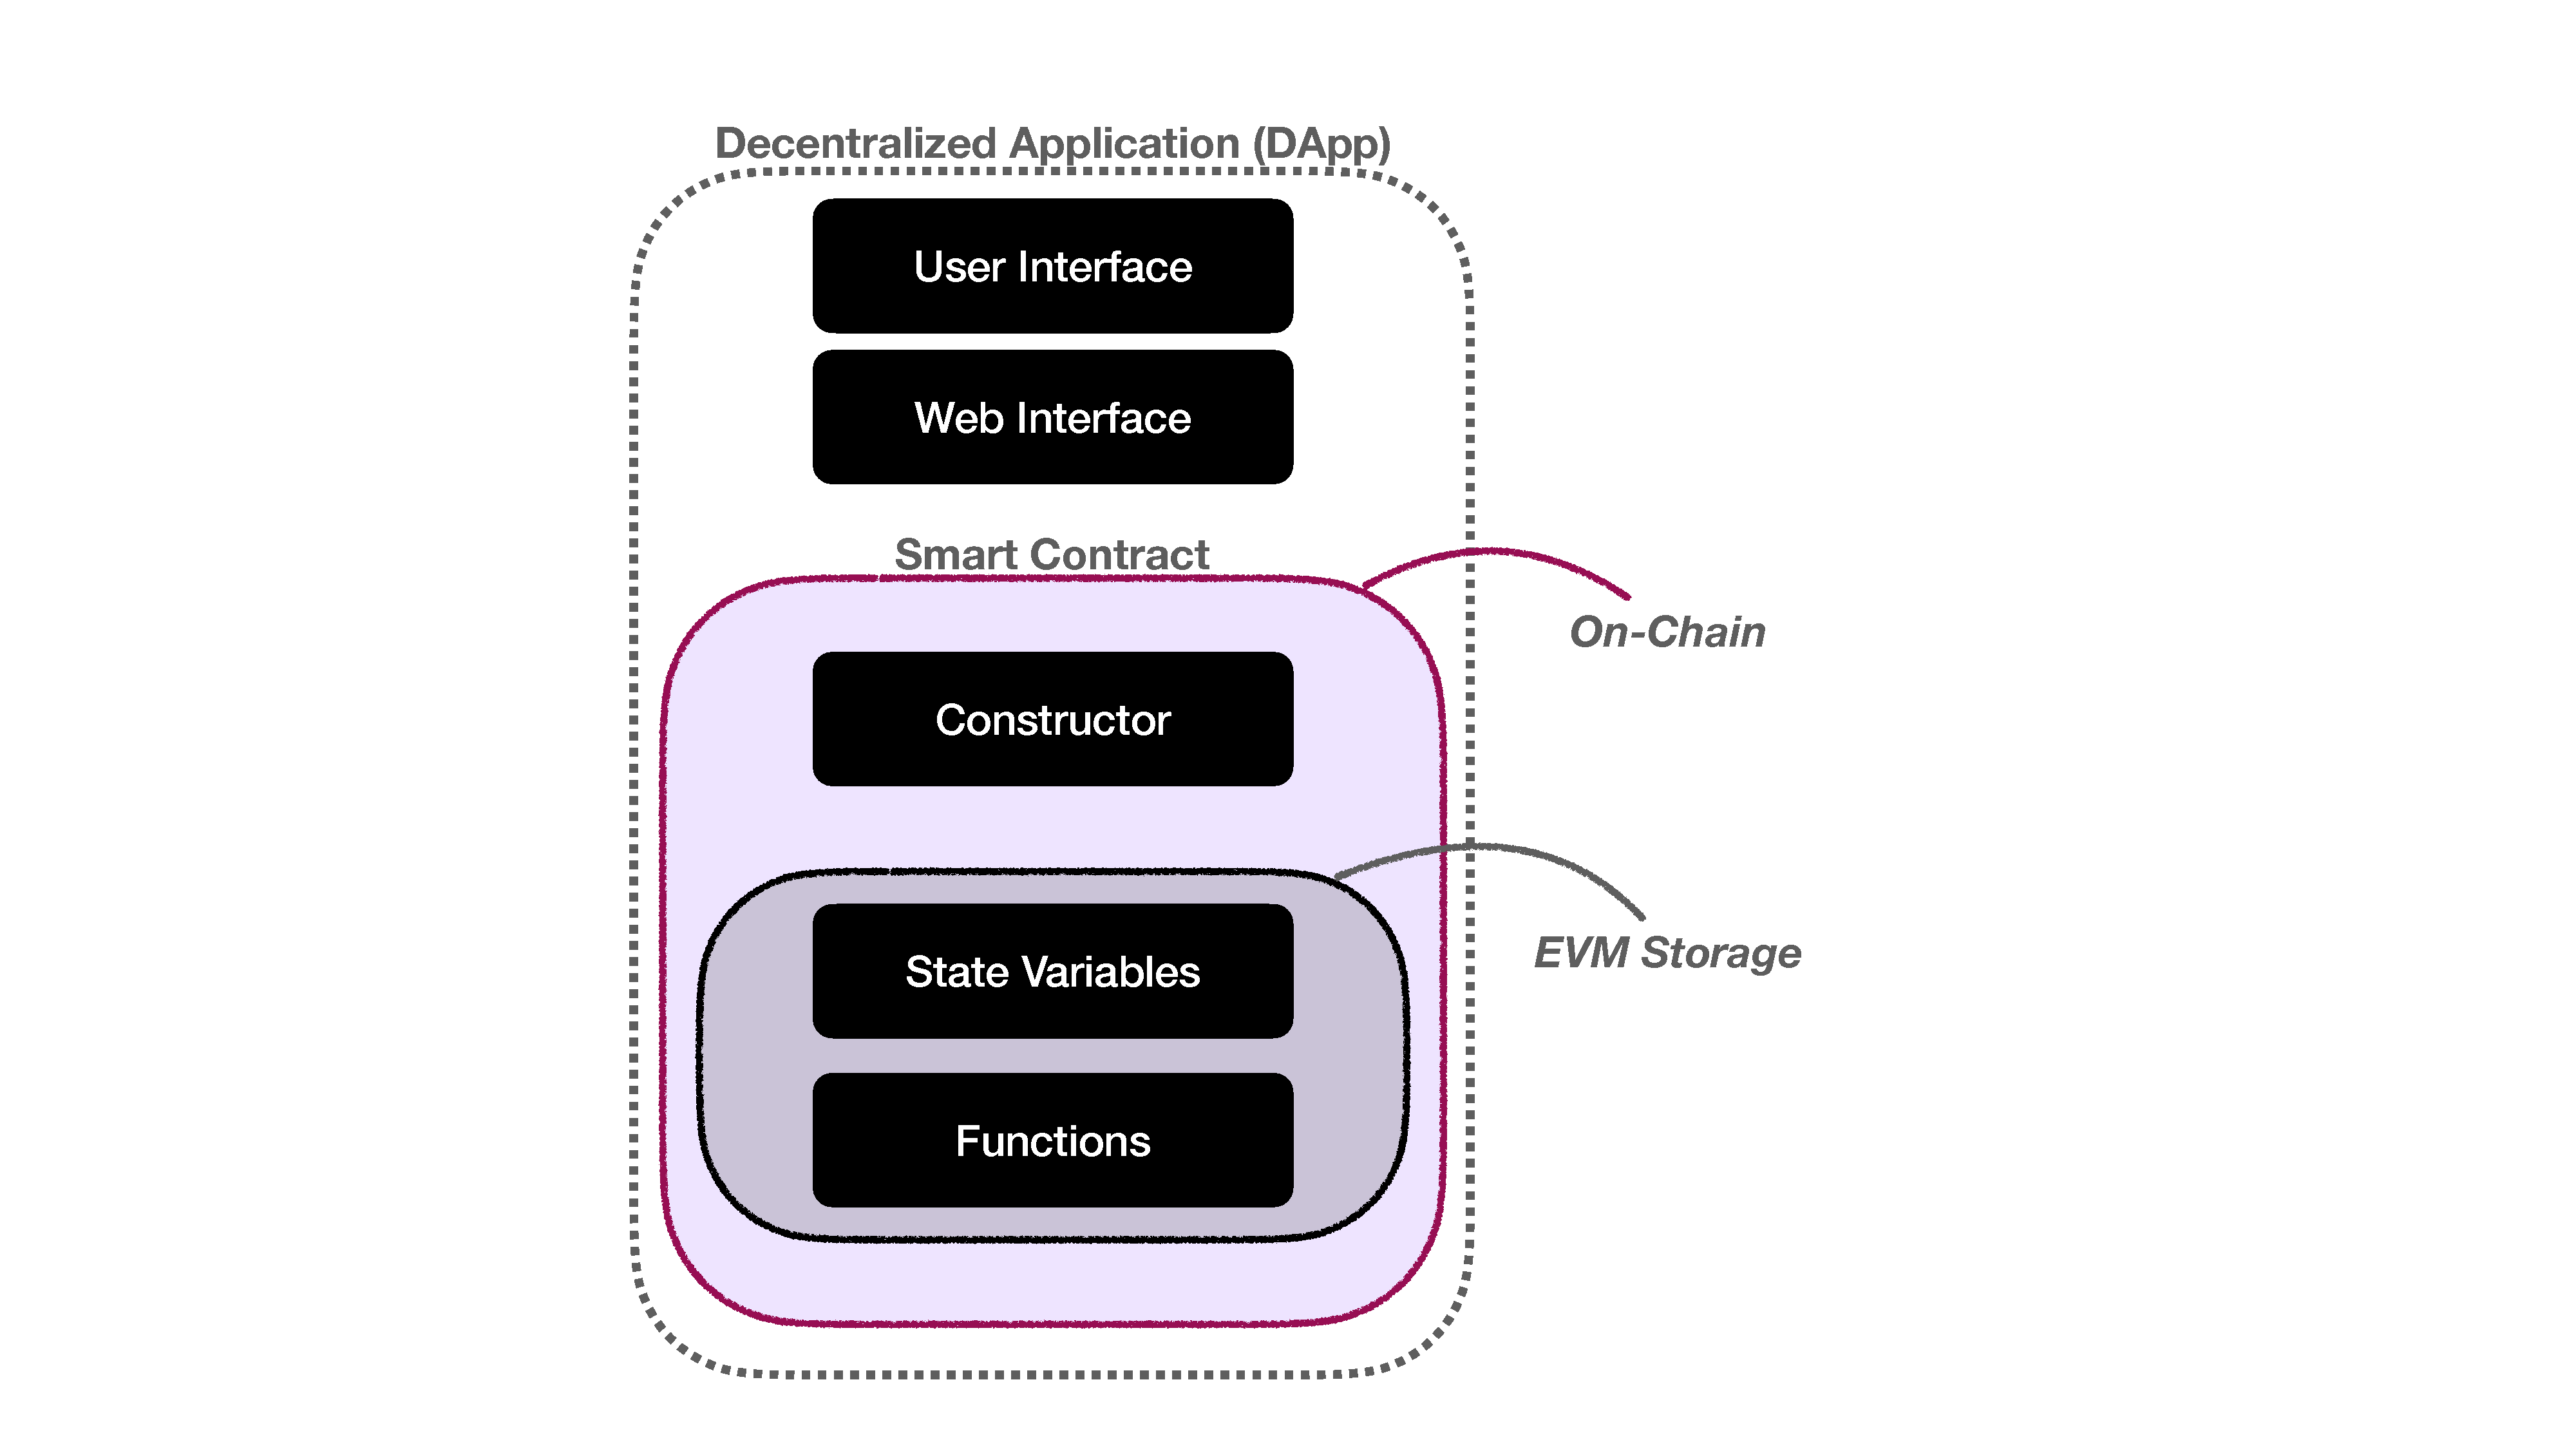
\includegraphics[width=0.4\textwidth]{figures/dapp.pdf}
  \caption{Components of a decentralized application.\label{fig:dapp}}
 \end{figure}

\paragraph{Updating vs. upgrading.} Software maintenance is part of software's lifecycle, and the process of changing the product after delivery. Often a distinction is drawn between software \textit{updates} and software \textit{upgrades}. An update modifies isolated portions of the software to fix bugs and vulnerabilities. An upgrade is generally a larger overhaul of the software with significant changes to features and capabilities. In our paper, we will only use the term upgrade and instead distinguish between retail (parameters and isolated code) and wholesale (entire application) changes. 

\paragraph{DApp vs. smart contract.} Figure~\ref{fig:dapp} shows the main components of a decentralized application (DApp). The core component is the smart contract (or simply contract), which is the set of functions and state stored on-chain. When first deployed, the smart contract also includes a constructor function which executes once and is then discarded (to be more precise, a copy of the constructor is stored in the record of transactions, called the calldata, but it is not retained in the EVM and can never be called again). While it is possible to interact directly with a smart contract by invoking its functions through Ethereum, generally users are provided an off-chain website with a user interface. Website actions are translated into calls to the Ethereum network through a set of tools (most prominently web3) in the web interface. 

While upgrades to the user interface can significantly change a user experience and expose new features, they are governed by traditional software maintenance. Our paper only considers the on-chain smart contract component, which is significantly more challenging to upgrade as it is on-chain and immutable under reasonable circumstances. 

\paragraph{Related work.} \textblue{TBD}

% = = = = = = = = = = = = = = = = = = = = = = = = = = = = = = = = = = = = = = = = = =

\section{Classification of Upgrade Patterns}

\begin{figure}[t]
  \centering
      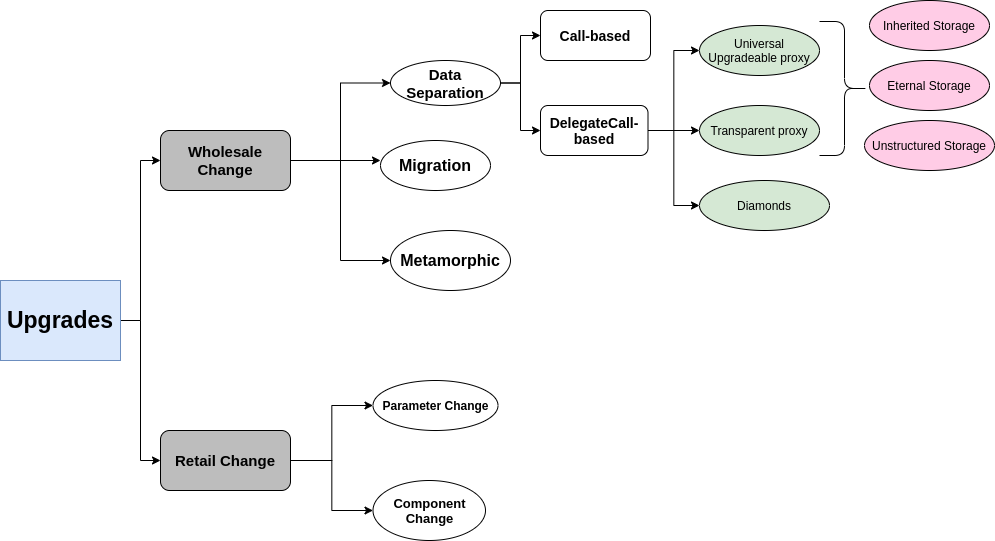
\includegraphics[width=0.8\textwidth]{figures/New_Classification.png}
  \caption{Classification. \textblue{Re-arrange to match ordering of text. Include section numbers of leaf nodes.}\label{fig:class}}
 \end{figure}
 
A variety of upgradeability patterns have been proposed for smart contracts on Ethereum. We categorize them in Figure~\ref{fig:class}. While some distinctions we make are applicable to other blockchain systems or even to software in general, the most popular approaches are leveraging Ethereum-specific operations and memory layouts.

The approaches have evolved over  time and some of them are no longer useful because of the advantages of other new methods. \textblue{Can we prove this with measurements?}

% Misc notes:
% We have some off-chain upgrades like what people did to force UNISwap using arbitrum as the L2 solution. It is an off-chain upgrade not an automated one.
% Does Factory patterns can be defined as upgradeability patterns? Like creating a new pool for Uniswap!


% JC: It seems the evaluation table will capture this. Plus are these pros/cons relative to each other or to other kinds of upgradeability (assuming the latter, it is hard to discuss until we have shown how they work). 
%The \textit{Pros and Cons} for retail changes methods are:
%\begin{itemize}
%  \item Pros
%  \begin{itemize}
%    \item Simple to implement
%    \item Easy to audit
%  \end{itemize}
%  \item Cons
%  \begin{itemize}
%    \item Cannot fix a bug
%    \item Cannot add/change Logic in Parameter Configuration
%    \item Cannot add new Logic in Tweak Strategy
%  \end{itemize}
%\end{itemize}

% = = =

\subsection{Parameter Configuration}
\label{sec:parameter}

We first categorized upgradeability patterns into two main classes: \textit{retail changes} and \textit{wholesale changes}. A pattern for retail change does not enable the replacement of the entire contract. Rather, a component of the contract is pre-determined (before the contract is deployed on Ethereum) to allow future upgrades, and the code is adjusted to allow these changes. 

The simplest upgrade pattern is to allow a system parameter, that is stored in a state variable, to be changed. This requires a \textit{setter function} to overwrite (or otherwise adjust) the variable, and access control over who can invoke the function. For example, in decentralized finance (DeFi), many services have parameters that control fees, interest rates, liquidation levels, \etc. Adjustments to these parameters can initiate large changes in how the service is used (its `tokenomics'). A DeFi provider can retain control over these parameters, democratize control to a set of token holders (\eg stability fees in the stablecoin project MakerDao), or lock the parameters from anyone's control. In Section~\ref{sec:governance}, we dive deeper into the question who can upgrade a contract. 

% = = =

\subsection{Functional Component Change}
\label{sec:component}

While a parameter change allows an authorized user to overwrite memory, a functional component change addresses modifications to the code of a function (and thus, the logic of the contract). In the EVM, code cannot be modified once written and so new code must be deployed to a new contract, but can be arranged to be called from the original contract. 

One way to allow upgradable functions is deploying a helper contract that contains the code for the functions to be upgradeable. Users are given the address of the primary contract, and the address of this secondary (helper) contract is stored as a variable in the primary contract. Whenever thhis function is invoked at the primary contract, the primary contract is pre-programmed to forward the function call, using the opcode \texttt{Call}, to the address it has stored for the secondary contract. To modify the logic of the function, a new secondary contract is deployed at a new address, and an authorized set of individuals can then use a parameter change in the primary contract to update the address of the secondary contract.

The DeFi lending platform Compound uses this pattern for their interest rate models which are tailored specifically for each asset. The model for one asset can be changed without impacting the rest of the contract.

Upgradeable functional components need to be pre-determined before deploying the primary contract. Once the primary contract is deployed, it is not possible to add upgradeability to existing (non-upgradable) functions. It also cannot be directly used to add new functions to a contract. Finally, this pattern is most straightforward when the primary contract only uses the return value from the function to modify its own state. Thus, the function is either `pure' (relies only on the parameters to determine the output) or `view' (can read state from itself or other contracts, but cannot write state). If the function modifies the state of the primary contract, the primary contract must either expose its state variables to the secondary contract (by implementing setter functions), or it can run the function using \texttt{DelgateCall} if the secondary contract has no state of its own. 

This upgrade pattern suggests a way forward for wholesale changes to the entire contract: create a generic `proxy' contract that forwards all functions to a secondary contract. To work seamlessly, this requires some further engineering (sections~\ref{sec:callbased} and \ref{sec:delegatecall}).

% = = =

% \paragraph{Pluggable Modules}. In this pattern we have a core contract that have some immutable features and then new contracts generated by the main contract and each have some or all features of the main contract. This pattern is mostly used in wallets and DeFi services like DeFi saver and InstaDapp. Users can decide to add new features into their wallet. 


%We need upgradeability to fix a bug or adding a new feature. In the event of fixing a bug, the agent who is responsible for the upgrade need to be as quick as possible to address a security issue or bug and so there is no need to have consensus of the users of the Dapp to make change. But, in the latter case the agent must get the consensus of the Dapp users to change and add a new feature, so they do not need to be quick. This fact is another paradox in the upgradeability of smart contracts because these two different events are not distinguishable before occurring and so we cannot implement two different ways of upgrading a system (one for resolving bug, and one for adding feature). So, as a system designer, if decide to add upgradeability feature should select one of these as the main goal of adding upgradeability and design the system based on that.

% = = =

\subsection{Consensus Override}
\label{sec:hardfork}

The two previous patterns enable portions of a smart contract to be modified. The remaining patterns strive to allow an entire contract to be modified or, more simply, replaced. The first wholesale pattern is not a tenable solution to upgradeability as it as only been used rarely under extraordinary circumstances, but we include it for completeness. 

Immutability is enforced by the consensus of the blockchain network. If participating nodes (\eg miners) agreed to suspend immutability, they can in theory allow changes to a contract's logic and/or state. If agreement is not unanimous, the blockchain can be forked into two systems---one with the change and one without. In 2016, a significant security breach of a decentralized application called `the DAO' caused the Ethereum Foundation to propose overriding the immutability of this particular smart contract to reverse the impacts of attack. In the unusual circumstances of this case, it was possible to propose and deploy the fix before the stolen ETH could be extracted from the contract and circulated. Nodes with a philosophical objection to overriding immutability continued operating, without deploying the fix, under the name Ethereum Classic.
%Need to talk about L2 (Roll-ups) --> They can roll-back the chain state similar to the DAO fork (they can setup new desired rollup state and bridge regarding that).
%\textbf{Upgradeability is a Bug!}~\cite{Upg-Bug}.


% = = =

\subsection{Contract Migration}
\label{sec:migration}

The simplest wholesale upgrade pattern is to deploy a new version of the contract at a new address, and then inform users (and the web applications they use) to use the new version---called a `social upgrade.' One example is Uniswap, which is on version 3 at the time of writing. Versions 1 and 2 are still operable at their original addresses. 

Contract migration does not require developers to instrument their contracts with any new logic to support upgradability, as in many of the remaining patterns, which can ease auditability and gas costs for using the contract. However for most applications, there will be a need to transfer the data stored in the old contract to the new version. This is generally done in one of two ways. The first is to collate the state of the old contract off-chain and load it into the new contract (\eg via its constructor). If the old contract was instrumented with an ability to pause it, this can eliminate race-conditions that could otherwise be problematic during the data migration phase. The second method, specific to certain applications like tracking a user's balance of tokens, is to have the user initiate (and pay the gas) for a transfer of their balance from the old system to the new one.
 
 % JC: do we *need* one or it is useful?
 %Also we need a \textit{Migrator} contract if we decided to outsource the data migration into the users.
 
 % = = =

\subsection{\texttt{CREATE2}-based Metamorphosis}
\label{sec:metamorphic}

Is it possible to do contract migration, but deploy the new contract to the \textit{same} address as the original contract, effectively overwriting it? If so, developers can dispense with the need for a social upgrade (but would still need to accomplish data migration). At first glance, this should not be possible on Ethereum, however a set of opcodes can be `abused' to allow it: specifically, the controversial\footnote{\href{https://www.reddit.com/r/ethereum/comments/lx32kv/expectations\_for\_backwardsincompatible\_changes/}{``Expectations for backwards-incompatible changes / removal of features that may come soon.'' V. Buterin, Reddit r/ethereum, Mar 2021.}} \texttt{SELFDESTRUCT} opcode and the 2019-deployed \texttt{CREATE2}. 

Consider a contract, called Factory, that has the bytecode of another contract, A, that Factory wants to deploy at A's own address. \texttt{CREATE2}, which supplements the original opcode \texttt{CREATE}, provides the ability for Factory to do this and know in advance what address will be assigned to contract A, invariant to when and how many other contracts that Factory might deploy.  The address is a structured hash of A's ``initialization'' bytecode, parameters passed to this code, the factory contract's address, and a salt value chosen by the factory contract.\footnote{Specifically: $\mathsf{addr} \leftarrow \mathcal{H}(\mathtt{0xff} \| \mathsf{factoryAddr} \| \mathsf{salt} \| \mathcal{H} (\mathsf{initBytecode} \| \mathsf{initBytecodeParams}))$} Most often, A's initialization bytecode contains a copy of A's actual code (``runtime'' bytecode) to be stored on the EVM, and the initialization code is prepended with a simple routine to copy the runtime code from the transaction data (calldata) into memory and return. Importantly, however, the initialization bytecode might not contain A's runtime bytecode at all, as long as it is able to fetch a copy of it from some location on the blockchain and load it into memory. In order for \texttt{CREATE2} to complete, the address must be empty, which means either (1) no contract has ever been deployed there, or (2) a contract was deployed but invoked \texttt{SELFDESTRUCT}.

%It is also common that A's initialization code will initialize some of A's storage variables (\eg the code specified in the constructor function in Solidity) using parameters passed into it. 

%The initialization bytecode passed to \texttt{CREATE2} will be recorded in the transaction call and then executed, but it is not stored in contract A. The expected result of executing the initialization bytecode is that contract A's runtime bytecode will be deployed at the determined address. 

Assume the developer wants to deploy contract A using metamorphosis and later update it to contract B.\footnote{\href{https://medium.com/@0age/the-promise-and-the-peril-of-metamorphic-contracts-9eb8b8413c5e}{``The Promise and the Peril of Metamorphic Contracts.'' 0age, Medium, Feb 2019.}} The developer first deploys a factory contract with a function that accepts A's (runtime) bytecode as a parameter (which includes the ability to self destruct). The factory then deploys A at an arbitrary address and stores the address in a variable called codeLocation. The factory then deploys a simple `transient' contract using \texttt{CREATE2} at address T. This contract performs a callback to the factory contract, asks for factory.codeLocation, and copies the code it finds there into its own storage for its runtime bytecode and returns. As a consequence, A's bytecode is now deployed at address T. 

To upgrade to contract B, the developer calls \texttt{SELFDESTRUCT} on A. It then calls the factory with contract B's bytecode. The factory executes the same way placing a pointer to B in factory.codeLocation. Importantly, it generates the same address T when it invokes CREATE2 since the `transient' contract is identical to what it was the first time---this contract does not contain contract A or B's runtime code, it just contains abstract instructions on how to load code. The result is contract B's runtime bytecode being deployed at address T where contact A was. 
 
% JC: Not important enough to keep:
%One limitation of this pattern is that Contract A and B cannot make use of a constructor, as the constructor is utilized by the transient contract. However contract A and B can implement a constructor-esque function that the factory invokes after \texttt{CREATE2} and  modifiers in the contract enforce it is only executable once. The only tangible difference is that its code will be stored as part of its runtime bytecode, whereas real constructor code is executed once and discarded (it is still recorded in the calldata of the transaction that creates the contract). 

As it is concerning that a contract's code could completely change, we note that metamorphic upgrades can be ruled out for any contract where either: it was not created with \texttt{CREATE2}, it does not implement \texttt{SELFDESTRUCT}, and/or its constructor is not able to dynamically modify its runtime bytecode. 

%This type of upgradeability is relevant to \textit{Create2} opcode which is proposed by Vitalik Buterin in 2018-04-20 as EIP-1014. To create a new contract in Ethereum blockchain we have 2 different opcodes; Create and Create2. The main difference between these two is the address of the contract that is going to be deployed. In Create opcode the address depends on the address and nonce of the creator. Nonce is a number regarding to the account and is like a counter to the number of transactions sent by that account (for contract account nonce is the number of contracts that are deployed by that contract). The problem of using Create opcode for contract deployment is that we cannot have a way to calculate the address of deployed contract because it depends on the nonce of the sender. Create2 opcode solve this problem because the address of the deployed contract just depends on the address of deployer and the \textit{Bytecode} of the contract to be deployed (and also a salt number which the deployer should specify each time). So we can hardcode the address of the deployed contract before deployment if we uses Create2.


%$\mathsf{addr} \leftarrow \mathcal{H}(\mathtt{0xff} \| \mathsf{facoryAddr} \| \mathsf{salt} \| \mathcal{H} (\mathsf{bytecode} \| \mathsf{owner} \| \mathsf{constructorParams}))$


%The other important property of Create2 opcode is that it uses \textit{init code} as the bytecode to calculate the address for deployment. The init bytecode is the bytecode which the creator will send to Ethereum blockchain and it is different from the \textit{Runtime Bytecode}. In fact, the EVM will execute constructor before deployment of the contract and then change the bytecode to the runtime code so the main difference between init bytecode and runtime bytecode is the constructor.

%In Metamorphic upgrade pattern, we abuse the Create2 opcode and take advantage of the difference between init bytecode and runtime bytecode to redeploy a contract with a new logic in the same address. To describe the process completely we should describe the Metamorphic Contract Factory a bit. This factory contract clones the implementation contract in its constructor and deploy the new bytecode on the previous address. The key idea is that the bytecode that we are going to deploy has a constructor that changes the bytecode to what we want to be deployed. So the init bytecode is the same as the previous deployment but the runtime bytecode is the new bytecode that we want to deploy.

%There is a critical point here. Before deploying a new contract on that exact address, the previous contract should be self destructed. Note that self destruct will wipe out the storage of the contract. So, in metamorphic upgradeability pattern we will lose the data and so we should migrate the data manually after deployment. In fact this type of upgradeability pattern is good for stateless contracts or contracts that has a limited storage variables (e.g. Beacon contract). The greatest risk to this type of upgradeability pattern is that there is a huge debate on the Ethereum community to remove the self-destruct opcode and without the self-destruct opcode the pattern is broken. 

% JC: will compare after discussion proxy patterns
%In comparison to the proxy patterns, metamorphic pattern is more gas efficient because we don't need to have any checks like what we had in transparent proxy or also we don't have the delegate call process. Similar to proxy contract, after upgrade the address of new version is not changed but we need to migrate the old data to the newer version. Also in metamorphic pattern there is downtime to the system because we should firs self-destruct the previous contract and the process of self-destructing occurs at the end of the transaction. So, we should first self-destruct the old version in a transaction and then redeploy the contract in another transaction and there is a downtime between these 2 transactions.


% = = =

\subsection{\texttt{CALL}-based Data Separation}
\label{sec:callbased}

To avoid moving the stored data from a contract to an upgraded contract, a contract could instead store all of its data in an external ``storage'' contract. In this pattern, calls are made to a ``logic'' contract which implements the function (or reverts if the function is not defined). Whenever the logic contract needs to read or write data, it will call the storage contract using setter/getter (aka accessor/mutator) functions. An upgrade consists of (1) deploying a new logic contract, (2) pausing the storage contract, (3) granting the new logic contract access to the storage contract, (4) revoking access from the old contract, and (5) unpausing the storage contract. 

An important consideration is that the layout of the storage contract cannot be changed after deployment (\eg we cannot add a new state variable). This can be side-stepped to some extent by implemented a mapping (key-value pair) for each primitive data type. For example, a new uint state variable can be a new entry in the mapping for uints. This is called the Eternal Storage pattern (ERC930). It however requires that every data type be known in advance, and is challenging to use with complex types (\eg structs and mappings themselves).

A variant of this pattern can introduce a third kind of contract, called a proxy contract, to address the social upgrade problem. In this variant, users permanently use the address of the proxy contract and always make function calls to it. The proxy contract stores a pointer (that can be updated) to the most current logic contract, and asks the logic contract to run the function using \texttt{CALL}. Unlike the functional component pattern (Section~\ref{sec:component}), the proxy will catch and forward \textit{any} function (including new functions deployed in updated logic contracts) using its fallback function.  With or without proxies, this pattern is very powerful, but instrumenting a contract to use it requires deep-seated changes to the contract code. As our measurements will show, it has fallen out of favour for the cleaner \texttt{DELEGATECALL}-based pattern (Section~\ref{sec:delegatecall}) that addresses the same issues with simpler instrumentation. 

% JC: already covered by contract migration :
%In this type of upgrade the address of the contract will be changed after upgrade so we need to aware our users about the change and interacting with the new version. Also it may break the compatibility of the ecosystem. In case of upgrade all smart contracts and Dapps that are interacting with the upgraded smart contract must change the address which they pointed to in order to interact with our contract. It may leads into a disaster if other contracts that are interacting with our contract do not have a way to change the address. We should also make other off-chain services (e.g. exchanges) aware of the change to start using the new version of your contract. In Call-based pattern we should have a way to stop previous version during/after upgrade because both of them are shared the same storage contract. 

% JC: this is covered I think
%There are three main ways to implement upgrades using data separation pattern. The easiest way is to change the ownership of storage contract into new upgraded logic contract and then \textit{Pause} the old contract using \textit{Circuit Breaker} pattern or set its pointer to 0x0 address. The other solution is to forward the calls receive by the old contract into the new logic contract. The last option is to set a registry contract that just keeps the address of latest version of the logic contract and call into it.

% JC:  Save evaluation for the table
% Using Calls-based pattern we eliminate the process of data migration from the old contract to the newer version and it is easy to understand this type of upgradeability pattern. But it is hard for developers to deal with this pattern when their logic contract needs complex data structures such as mapping or structures. Also the developers should change their code a lot if they decide to use this upgradeability pattern in their non-upgradeable code. 

% = = =

\subsection{DelegateCall-based Data Separation}
\label{sec:delegatecall}
%In this pattern, a typical function call is chained through three contracts. The call is always made to the same contract, called the proxy contract, that is deployed permanently at a given address. The proxy contract stores a pointer to a second contract, called the logic contract, and implements only a few basic functions (\eg for updating the pointer). Any function (with any other function name) that is invoked is caught by the contract's fallback function and forwarded with the parameters, using \texttt{CALL}, to the logic contract. 

%function () payable public {
%        address target = logic_contract;
%        assembly {
%            let ptr := mload(0x40)
%            calldatacopy(ptr, 0, calldatasize)
%            let result := delegatecall(gas, target, ptr, calldatasize, 0, 0)
%            let size := returndatasize
%            returndatacopy(ptr, 0, size)
%            switch result
%            case 0 { revert(ptr, size) }
%            case 1 { return(ptr, size) }
%        }

Similar to call based patterns here we have two contracts, Storage and Logic contract. In this pattern we may have more than one logic contract or storage contract. The difference here is that the user is calling storage contract(s) first (a.k.a proxy contract), and the proxy contract will use \textit{DelegateCall} opcode to link to the logic contract(s) (a.k.a implementation contract). In fact, there is a fallback function inside the proxy contract and inside the proxy, there is a delegate call that forwards the whole message data to the implementation contract.
The fallback functions in Ethereum will be executed if the user calls the smart contract with a function signature that does not exists on that contract.

So, if the user calls a function that does not exists on the proxy contract, the fallback will be executed and so the message data will be delegated call into the implementation contract and if the function that is called by user exists on the implementation contract the function will be executed.

So if we need to add/change the functionality of our Dapp, we just need to deploy a new implementation contract and then change the implementation address inside the proxy contract to delegate call to the new version of the implementation.

Using this pattern has two major limitations that we should take care of:

First, as described above the pattern has an assumption that the function signature of the functions inside the implementation is not existed inside the proxy contract as well. Otherwise when a user calls that function the fallback function won't be executed because the function exists on the proxy contract. So that function is not achievable inside the proxy. In Ethereum when we want to call a function we just use 4 Bytes of the hash of function name and input/output types as the function signatures. So it is possible to have 2 completely different functions with the same function signature. In the case that we have a function in implementation contract that has the same function signature with one of the functions inside the proxy we say that function signature clashes happened.

Second, the delegatecall opcode in Ethereum will run the logic of the implementation contract in the context of the proxy contract. It is similar to copy pasting the logic code into the proxy contract and altering the storage of the proxy contract. Because the delegate call opcode preserves the context, we should be sure that the storage layout of the proxy contract and the logic contract should be the same. Otherwise when we try to change a storage slot in proxy, we will end up with changing another one. The difference between storage layouts will result in a storage clashes. 


Different proxy patterns are proposed to mitigate function selector clashes and storage clashes. We will describe each of them and the advantage and disadvantages of each of them.

The first problem that we should deal with in proxy contracts is function selector clashes. In fact inside the proxy contract we need just one function called \textit{upgradeTo} function that gives the owner of the contract ability to change the address of the implementation contract inside the proxy. So in the event of the upgrade, the owner will deploy the new implementation contract and change the address variable inside the proxy to the address of the newly deployed implementation contract. By doing this the fallback function will delegate call into the newer version. So to mitigate the problem of function signature clashing we should be sure that we do not have a function with function signature equal to the functions inside the proxy, we have two main approaches to mitigate this problem:

\paragraph{Universal Upgradeable Proxy Standard (UUPS)}. 
The Universal Upgradeable Proxy Standard (UUPS) method is proposed on 2019-03-04 and suggested to move the upgradeTo function to the implementation contract. So by doing this we do not have any function inside the proxy and the function signature will be mitigated. Also we reduced the size of the proxy contract. If the owner decides to upgrade the system, should call the upgrade function via calling the proxy and because the code is executed in the context of the proxy contract, the address variable of implementation inside the proxy contract will be changed.
There is a huge risk in using the UUPS proxy pattern. If the owner upgrades to a contract that does not implemented an upgradeTo functionality inside it, then the contract cannot be upgraded after that last upgrade because there is not any function inside the proxy and the latest implementation contract to upgrade the system. There is a way to check if the proposed address is a contract address and also the upgradeTo function is implemented inside that or not but that does not guarantee that the logic of the upgradeTo function is what needed to be.


\paragraph{Transparent Proxy}. 
The other way to mitigate the function clashes is to check the sender of the transaction. If the owner of the contract calls the proxy the upgrade function will be executed and otherwise the fallback will be executed. This way we are sure that even if we have function clashes, then user's call will be forwarded to the implementation. 
The drawback of using Transparent proxy is that we add a check for each call to the contract which added gas cost for users on each call to the contract. (it needs to first read the address of the owner from storage which needs high amount of gas and then a check that if the sender is owner or not). 


There are three different methods to mitigate the risk of storage clashes.  To mitigate storage clashes we have three different approaches :

\paragraph{Inherited Storage}. 
In this method the proxy and all logic contracts are inherited from a storage contract that contains storage variables. If we decided to upgrade the contract, we should be sure that the new implementation contract is inherited from the storage contract. Using this method we are confident that the proxy and logic contracts are using the same storage layout and storage clashes will be mitigated.
Also if after deployment we need to add new storage variables, we should just deploy a new storage contract that inherited from the previous storage contract and add the new variables to it. We should be sure that the future implementation contracts will inherit the latest storage contract. This adds-on to the inherited storage contract is called append-only pattern.
This method is not efficient because of variables that declared but not used in some logic contracts. On the other hand, each logic contract is coupled with a storage contract and it is hard to take care of this track. Also we should take care of upgrading the system each time to be sure that the new implementation contract is inherited from the latest version of storage contract.

\paragraph{Eternal Storage}. 
As described before in Eternal storage, we defined mappings for all variable types that we need to use in our logic smart contract. For storing mapping variables EVM selects random slots on the storage based on the variable's name so we can mitigate the clashes using this randomness.
The main problem of this type is that the logic contract and all other contracts that are using the storage must use the mapping structure to access the storage variables and use complex syntax whenever they want to access a variable. This also results in the gas usage inefficiency because we need to call and update a mapping each time we need to change a variable.  


\paragraph{Unstructured Storage}. 
The other way of mitigating the storage clashes is to assign some randomly selected slots to critical variables like address of logic contract. For instance, openzeppelin uses hash of "org.zeppelinos.proxy.implementation" to store the address of the logic contract in this slot.
The downside of this approach is that we need getter and setter function for each variable. We also can use unstructured storage for simple variables and not for mapping and structures. EIP-1967 proposed to assign specific storage slots for address variable inside the proxy contract to store the address of the implementation contract inside the proxy. The proposed slot is 0x360894a13ba1a3210667c828492db98dca3e2076cc3735a920a3ca505d382bbc which is calculated from this equation
bytes32(uint256(keccak256(eip1967.proxy.implementation)) - 1)). 
%% Add exact gas cost from the image

There are two other upgradeable proxy patterns that are proposed to address problems in some specific applications. We will describe them bellow: 

\paragraph{Beacon Proxy}. 
In some type of applications such as wallets, the logics needs to make the data of each user separate. There are some proposals such as EIP-1167 or minimal proxy suggested creating a proxy contract for each user that delegate calls to the main implementation contract. Using this approach each user has its own data inside its proxy contract. The problem of using the minimal proxies is that they are not upgradeable. If a bug found in the implementation contract then all proxy instances are prone to the attack. The problem of using the previous types of the upgradeability patterns is that unlike the previous ones that have just one proxy contract and easy to change the address variable inside them, here we have tons of instances and we cannot change all address variables inside all proxies. 

Beacon proxy method is suggested to solve this issue. In beacon proxy, each proxy instance will call a registry-like contract and ask it for the latest version of the implementation contract and then will delegatecall to the resolved address. In the upgrade event, the owner needs to just change the address inside the beacon contract so all proxy instances will use the newer version of implementation contract each time calling the beacon contract and asking for the implementation contract address.

\paragraph{Diamonds}
The EIP-2535 or Diamonds proxy is proposed on 2020-02-22 and suggested using multi implementation contracts with a single proxy contract. In the proxy there is a access control structure in which there is a mapping between each implementation contract's address and the function signatures that are implemented inside that specific implementation contract. Using this method we can have a separate implementation contract for each functionality of the Dapp. It will help to make the contracts more modularize. Also we can just update one functionality in each upgrade event. It also helps with the situation that the contract code size exceeds the limitation (24KB) by splitting it into a number of implementation contracts.

The drawback of using Diamonds is adding more complexity to the system because using different implementation contracts will increase the chance of storage clashes and error in handling the shared storage between them.




\subsection{Evaluation Framework}
% !TEX root = ../main.tex

\begin{table}[t!]
    \centering
    
        \begin{tabular}{lllllllllllllll}
    
    &
    \headrow{Can replace entire logic} &
    
    \headrow{can replace pre-specified part of logic} & 


    \headrow{Can replace entire state} &
    
    \headrow{can change pre-specified state variables} &
    
    \headrow{No need to deploy a new contract} &

    \headrow{No need to migrate state from old contract} &

    \headrow{No need to separate State and Logic} &

    \headrow{Function Selector Clashes Risk} &

    \headrow{Storage Clashes Risk} & 

    \headrow{No indirection} & 


    \headrow{User endpoint address not changed} &
    

    \headrow{Downtime in upgrade events} &

    \headrow{No need to change code to add the upgrade pattern} &

    \headrow{Need to change a state variable} 
    
    
    \\
    
    \hline
 
    
        \multicolumn{1}{c|}{Parameter change}	& \multicolumn{1}{c|}{}  & \multicolumn{1}{c|}{} &  \multicolumn{1}{c|}{} & \multicolumn{1}{c|}{\checkmark} & \multicolumn{1}{c|}{\checkmark} & \multicolumn{1}{c|}{\checkmark} &  \multicolumn{1}{c|}{\checkmark} &  \multicolumn{1}{c|}{} & \multicolumn{1}{c|}{} & \multicolumn{1}{c|}{\checkmark} & \multicolumn{1}{c|}{\checkmark} & \multicolumn{1}{c|}{} &\multicolumn{1}{c|}{\checkmark} & \multicolumn{1}{c}{\checkmark}\\
    
        \hline
  
        \multicolumn{1}{c|}{Component Change}	& \multicolumn{1}{c|}{}  & \multicolumn{1}{c|}{\checkmark} &  \multicolumn{1}{c|}{} & \multicolumn{1}{c|}{} & \multicolumn{1}{c|}{} & \multicolumn{1}{c|}{\checkmark} &  \multicolumn{1}{c|}{\checkmark} &  \multicolumn{1}{c|}{} &  \multicolumn{1}{c|}{} &  \multicolumn{1}{c|}{\XBox} & \multicolumn{1}{c|}{\checkmark} & \multicolumn{1}{c|}{} & \multicolumn{1}{c|}{\XBox} &  \multicolumn{1}{c}{\checkmark}\\
        

        \hline

        \makecell{Migration}	& \multicolumn{1}{|c|}{\checkmark}  & \multicolumn{1}{c|}{} &  \multicolumn{1}{c|}{\checkmark} & \multicolumn{1}{c|}{} & \multicolumn{1}{c|}{} & \multicolumn{1}{c|}{} &  \multicolumn{1}{c|}{\checkmark} &  \multicolumn{1}{c|}{} &  \multicolumn{1}{c|}{} &  \multicolumn{1}{c|}{\checkmark} & \multicolumn{1}{c|}{} & \multicolumn{1}{c|}{} & \multicolumn{1}{c|}{\checkmark} &  \multicolumn{1}{c}{}\\
    
         \hline


        \makecell{Call-based}	& \multicolumn{1}{|c|}{\checkmark}  & \multicolumn{1}{c|}{} &  \multicolumn{1}{c|}{} & \multicolumn{1}{c|}{} & \multicolumn{1}{c|}{} & \multicolumn{1}{c|}{\checkmark} &  \multicolumn{1}{c|}{} &  \multicolumn{1}{c|}{} &  \multicolumn{1}{c|}{} &  \multicolumn{1}{c|}{} & \multicolumn{1}{c|}{} & \multicolumn{1}{c|}{} & \multicolumn{1}{c|}{} & \multicolumn{1}{c}{\checkmark}\\
    
        \hline


        \makecell{DelegateCall-based}	& \multicolumn{1}{|c|}{\checkmark}  & \multicolumn{1}{c|}{} &  \multicolumn{1}{c|}{} & \multicolumn{1}{c|}{} & \multicolumn{1}{c|}{} & \multicolumn{1}{c|}{\checkmark} &  \multicolumn{1}{c|}{} &  \multicolumn{1}{c|}{\checkmark} & \multicolumn{1}{c|}{\checkmark}&  \multicolumn{1}{c|}{} & \multicolumn{1}{c|}{\checkmark} & \multicolumn{1}{c|}{} & \multicolumn{1}{c|}{\XBox} & \multicolumn{1}{c}{\checkmark}\\

        \hline

        \makecell{Diamonds}	& \multicolumn{1}{|c|}{\checkmark}  & \multicolumn{1}{c|}{} &  \multicolumn{1}{c|}{} & \multicolumn{1}{c|}{} & \multicolumn{1}{c|}{} & \multicolumn{1}{c|}{\checkmark} &  \multicolumn{1}{c|}{} &  \multicolumn{1}{c|}{\checkmark} & \multicolumn{1}{c|}{\checkmark\checkmark}&  \multicolumn{1}{c|}{} & \multicolumn{1}{c|}{\checkmark} & \multicolumn{1}{c|}{} & \multicolumn{1}{c|}{\XBox} & \multicolumn{1}{c}{\checkmark}\\
        
        
         \hline

        \makecell{Metamorphic}	& \multicolumn{1}{|c|}{\checkmark}  & \multicolumn{1}{c|}{} &  \multicolumn{1}{c|}{\checkmark} & \multicolumn{1}{c|}{} & \multicolumn{1}{c|}{} & \multicolumn{1}{c|}{} &  \multicolumn{1}{c|}{\checkmark} &  \multicolumn{1}{c|}{} & \multicolumn{1}{c|}{}&  \multicolumn{1}{c|}{\checkmark} & \multicolumn{1}{c|}{\checkmark} & \multicolumn{1}{c|}{\checkmark} & \multicolumn{1}{c|}{\checkmark} &  \multicolumn{1}{c}{}\\
        
        
         \hline
        
        
        \end{tabular}
        \captionsetup[tabular]{singlelinecheck=off}
        \caption{Evaluation}
       
    
    \end{table}
    \footnotetext[1]{Design of system in which a parameter can change the logic is hard}

Table~\ref{tab:eval} summarizes the pros and cons of each upgradability pattern. The details of the evaluation are provided in the full version of this paper.\footnote{To be archived. Can be provided anonymously though program chairs.}




 %%%%%%%%%%%%%%%%%%%%%%%%%%%%%%%%%%%%%%%%%%%%%%%%%%%%%%%%%%%%%%%%%%%%%%%%%%%%%%%%%%%%%%%%%%%%%%%%%%%%%%%%%%%%%%%%%%%%%%%%%%%%%%%%%%%%%%
 %%%%%%%%%%%%%%%%%%%%%%%%%%%%%%%%%%%%%%%%%%%%%%%%%%%%%%%%%%%%%%%%%%%%%


 \section{Finding Upgradeable Contracts on Ethereum}

 This section aims to shed light on the state of upgradeable smart contracts on the Ethereum blockchain. Between all the different patterns described in previous sections, we focused on finding the \textit{Delegate-call} based upgradeable contracts because it is the most widely used pattern for smart contract upgradeability at the time of writing this paper. The number of Ethereum Improvement Proposals (EIPs) and standards proposed for standardizing this pattern (e.g., EIP-1967, EIP-1822, EIP-2535, etc.) confirms this point. In the further parts of this section, we focus on describing the methodology used for finding upgradeable contracts in Ethereum blockchain, which use \textit{Delegatecall-based} patterns and show the results. \textblue{I have commented the detailed reason for choosing DelegateCall based pattern but removed it from the paper to summarize it}
%Here I have the reason why we chose delegate call based patterns:

%There is no general way to detect \textit{Retail Change} patterns in large-scale, in which one or multiple state variables can be changed inside the contract by admin of the contract, because there is no general way to distinct between a changeable state variable inside a contract that can be updated and non-critical one. It really depends on the business logic of the smart contract.

%\textit{Wholesale change} approaches consist of \textit{Call-based}, \textit{Delegatecall-based} and \textit{Metamorphic} patterns. The Call-based pattern is an old fashion way of adding upgradeability to a system. This type is not widely used nowadays. On the other hand, \textit{Delegate-call}  pattern is the most-used pattern in ethereum contracts and this is why we focused on this pattern in our research. \textit{Metamorphic} pattern is very new and not well-tested yet. Also it has limitations such as the state of the contract should wiped out before upgrade each time because of need of self-destruction. Also there are some risks to this pattern. For instance there are discussions in Ethereum community about removing \textit{Selfdesctruct} opcode from EVM~\cite{selfDestruct}. 

%In the above paragraph we claimed that the \textit{Call-based} pattern is not widely used these days. To prove this claim we perform an analysis on 93,000 verified smart contracts in smart contract sanctuary database~\cite{smart_contract_sanctuary} which gathers all verified smart contracts from \textit{Etherscan} blockchain explorer. As mentioned in previous sections \textit{Call-based} patterns consist of a logic contract and storage contract. The storage contract should define all storage variables needed for the system and must have getters and setters for these variables. Storage contract is the part that is not changing in upgrade events. So the developers should be sure that all state variables that are needed are defined in the deployment time or using tricks and patterns that give the developers ability to add new state variables after deployment. \textit{Eternal Storage} pattern is using a key-value based structure for the storage contract by using \textit{mappings} for defining all variables which gives the developers ability to add new variables after deployment. This is the reason that why Eternal Storage is widely used as the storage contract in \textit{Call-based} patterns. In this analysis, we try to find contracts that uses eternal storage structure in their logic using Regular Expression analysis. \emph{470} contract are found that uses eternal storage patterns and then we filtered them to find contracts that uses eternal storage structure and only contains getter and setter functions and not any other logics (the reason is described in the previous sections). After filtering we come up with \emph{170} unique eternal storage contracts that are used as storage contract of upgradeable Dapps. Checking the time of deployment of these contracts show that the latest one was deployed on July 2018 which show that this pattern is not widely used anymore these days (the reasons are discussed in the evaluation section).


\subsection{Methodology}
As mentioned in classification section, the \textit{DelegateCall-based} upgradeability approach consists of a storage contract (a.k.a proxy contract) and a logic contract (a.k.a implementation contract). 
The proxy contract is a simple type of smart contract in which there is a \textit{Fallback} function. Fallback is a function inside smart contracts that do not have a function name. If a user sends a transaction to a contract to call a function that does not exist, it will pass into the fallback function, and the logic inside the fallback function will be executed. So, calling a contract with a function signature that does not exist on that contract is equal to calling the contract's fallback function. Inside the fallback function of a proxy contract, there is a delegate call to the address of \textit{implementation contract} (we call it \emph{Target address} in the rest of the paper) which passes the whole data of the transaction to the implementation contract without altering it.

All proxy contracts have the above structure. However, \textit{Upgradeable proxy contracts} should have another extra condition as well. The agent who is responsible for changes in the smart contract (a.k.a \emph{admin}) must have the ability to change the target address. If a proxy does not have this condition, the contract delegates the data into a fixed implementation contract for the rest of its life. So, this type of proxies is not upgradeable. There are a bunch of patterns that follow this structure (e.g., Minimal Proxies~\cite{minimalProxy}, Delegate call forwarders~\cite{delegatecallForwarders}, etc.), which we call them \textit{Forwarders} in the rest of the paper. So, for upgradeable proxies, the target address must be \emph{changeable}.

To find the proxy contracts in Ethereum, we need to collect transactions and all information regarding those transactions. To collect the transaction details, we need to replay the transaction and collect the data of execution of the transaction. Ethereum full archival node has a method, \textit{trace\_transaction}, that gives the traces \footnote{Parity VM transaction trace} of the transactions executed on the specific block. We used this method to have transaction traces and find the transactions in which a delegate call happened. Each transaction trace may consist of several sub-traces (a.k.a, actions).
If the data of two consecutive sub-traces of a transaction are equal and a delegate call is in the second sub-trace, it shows that the transaction passes the fallback function. Because if any other function in the contract is called (other than fallback), then the first four bytes of the data will be changed. Also, a delegate call in the fallback transferred the whole data without altering it, which means the contract is a proxy contract.

As discussed above, these proxies can be forwarders or upgradeable proxies. To find upgradeable proxies, we should filter them by checking whether the target address variable is changeable or not. Three general standards are proposed to change the target address of a proxy; Beacon proxy, Regular proxy, and Universal Upgradeable proxy. 
As discussed in the classification part, the target address in beacon proxies comes from an external call to another contract named \textit{Beacon Contract}. So, to find upgradeable beacon contracts, we first check if the target address comes from an external call to another contract. If yes, we should check the callee contract to find out if the target address inside the beacon contract is changeable. If the target address is changeable, the proxy contract is a \textit{Beacon Proxy} contract, and the admin of the beacon contract can change the target address inside it to upgrade the system. 

If the address does not come from an external call, we check if there is any function inside the proxy contract that the admin can call to change the target address and upgrade the system. This is the most tricky part in our methodology to find out if a function inside the contract gives the admin the ability to change the target address. If that function is found, we mark the proxy as an upgradeable proxy contract. The process is divided into two main parts; 1) Finding the target storage variable regarding the target address, and 2) checking if there is an assignment to that specific storage variable inside the contract.

\textbf{Finding storage variable (slot) of the target address.} We use bytecode decompiler named \textit{Panoramix decompiler} \footnote{\url{https://github.com/palkeo/panoramix}} to decompile the bytecode of the contract into well-formatted python language codes. Then check to find the line of the code in which the delegate call happened and pick the target of the delegate call. We find the variable name or a storage slot of the target address, which is our goal in this part.

\textbf{Checking for assignment.} Now that we have the decompiled code and variable name (or storage slot) of the target address. We use the Regular Expression method to check if an assignment to that variable/slot happened in any function in the contract. If any assignment is found, we should be sure that the other variable assigned to the target address variable comes from the input of that function. If these conditions are satisfied, there is a function inside the contract that can change the target address and upgrade our system (upgrade function).

So by applying the first filter, we find the storage variable/slot of the target address and then check if it is changeable or not. If the target address is changeable, we mark the proxy as an upgradeable proxy contract.
If there is no way to change the target address inside the proxy, we pass it to another final filter. There is another way of implementing upgradeable contracts named \textit{Universal Upgradeable Proxy Standard (UUPS)} that is discussed in the classification section. In this method, the target address is changeable using the implementation contract. So to filter and find them, we check the implementation contract to find out if there is any function inside the implementation contract by which the admin can change the target address. If yes, then our proxy is a UUPS proxy contract. Otherwise, the proxy is not upgradeable. The first step here is to find the storage slot of the target address inside the proxy contract. Then we decompile the bytecode of the implementation contract and check to find if any assignment to that storage slot happened inside the implementation contract. The process of finding the assignment is very similar to the last part. So if a function is found that gives the admin a chance to write a new amount to the storage slot regarding the target address, the admin can call that function using the proxy to change the target address and upgrade the system. In this case, we marked the proxy as a UUPS proxy contract.
All the remained proxy contracts are marked as non-upgradeable proxy contracts. The whole process is depicted in figure~\ref{flowchart}. For a detailed explanation of the methodology and implementation, check the appendix.

\begin{figure}[t!]
  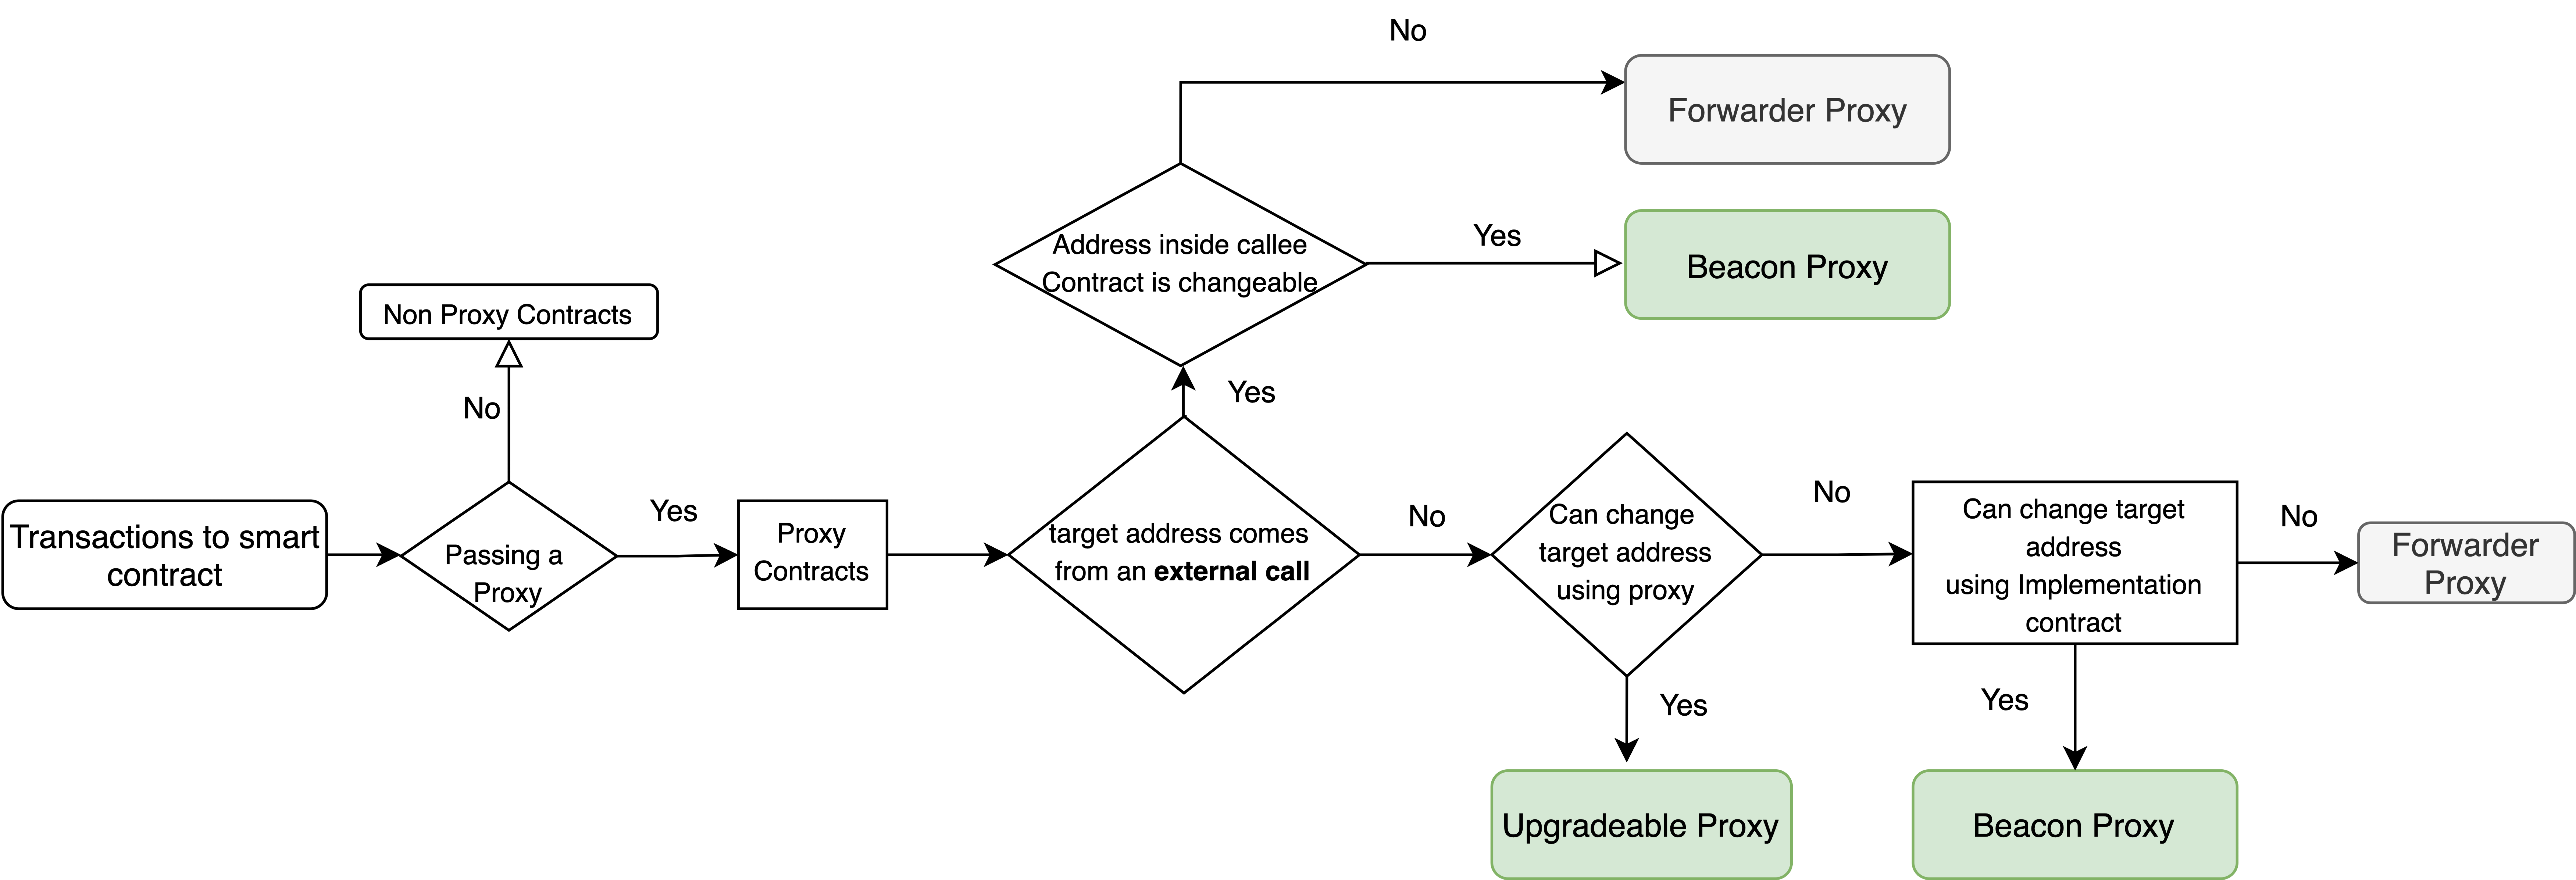
\includegraphics[width=1\textwidth]{New-method.png}\label{flowchart}
  \caption{Flowchart of the Process}
\end{figure}



\subsubsection{Results}

Having access to an Ethereum full archival node, we have collected transaction traces of transactions included in 2,064,595 blocks of Ethereum blockchain, starting from block number \textit{\#10800000} to \textit{\#12864595}. It covers transactions on the Ethereum blockchain from \textit{Sep-05-2020} to \textit{Jul-20-2021}. 

%Having transaction traces and the actions of each transaction, we have collected \textit{From} address (address of sender of the transaction), \textit{To} address (destination address of the transaction) and \textit{Transaction Hash} of actions which has \textit{delegateCall} as their \textit{Call Type} and their input is the same as their previous action. As mentioned in the previous part the From addresses are the address of the proxy contracts.

Applying our methodology gives us \textit{1,427,215} unique proxy contracts. However, a bunch of these proxies is using shared implementation contracts. We decide to weed out the proxy contracts that share the same implementation contract; however, two different Dapps may use the same implementation contract. The reason for this decision is that there are some Dapps like opensea~\footnote{\url{opensea.io}} that create proxy contracts for each of their user, and these proxies share the same implementation contract (it will reduce the redundancy). So after filtering proxies with the same implementation contracts, we come up with \textit{13,088} contracts.
Afterwards we filter \textit{Forwarder Contracts} from our dataset and totally we find \textit{7,470} regular upgradeable proxy contracts.
On the other hand, checking the remained proxy contracts and applying the methodology gives us \textit{403} upgradeable proxy contracts that follow Universal Upgradeable Proxy Pattern and also \textit{352} unique beacon proxy contracts.

At the end we find \textit{8,225} unique upgradeable proxy contracts with unique implementation contract. We randomly sampled 150 contracts from these contracts and manually checked them, and all of them were upgradeable proxy contracts. On the other hand, we sampled 150 contracts from those marked as non-upgradeable and checked them manually. Between these 150 contracts, just two were upgradeable, and it was a false-negative. Our model did not catch these contracts because a failure happened on the decompiler to decompile the implementation contract code, so our assignment checker detector could not catch them. The reason is that implementation contracts are huge codes in contrast with the proxy contract itself.


\section{Finding Admin of the Proxies}

This section proposes a novel way to find the admin of the proxy contract (the agent responsible for upgrading the proxy contract) and classify them based on their account type. We apply the method to the dataset we provided from the previous analysis. We also shed light on the risks regarding the number of decision-makers who have the authority to change the whole logic of the Dapps that are using a proxy contract.

The question we will answer in this part is who can upgrade the system? There should be an agent who decides on the upgrades of the system. Generally, there are three main types of admins for upgradeable smart contracts; a single Ethereum address (a.k.a EOA), Multi-Signature wallets, and Governance schemes. EOA and multi-signature schemes are adding Centralization to the system because a limited number of private keys can change the system's whole logic. Based on \textit{The State of DeFi Security 2021}~\cite{certikReport} report by Certik company~\footnote{\url{certik.com}}, \textbf{Centralization} is the most common attack vector of the hacked DeFi projects, so remaining a centralization point by permitting to change the system to some specific critical roles can be hazardous.
We are describing three types of admins below:

\textit{Externally owned Address(EOA)}
This most centralized way to deal with admin is to have just one private key control the upgrades. Using EOA as admin is the fastest way to respond to incidents, but in case of a malicious admin or a private key compromise, the whole funds are at risk.

\textit{Multi-Signature Wallet}
A \textit{m out of n} Multi-signature wallet is a smart contract that can execute a transaction only if m number out of a specified n EOAs agree and sign the transaction. 
Using multi-sig as admin is a better answer to the upgrade's decision-making than using an EOA in case of centrality while keeping the speed of an upgrade process. However, it is not decentralized. The problem here is that the Ethereum accounts are pseudo-anonymous, and the identity behind addresses is not recognizable. So, the malicious developer team can keep at least m signatures out of n in their hands, and in the desired time, they can upgrade a system to a malicious version and steal the funds.
Also, it is good to mention that there are some types of governance voting which is known by \textit{Off-chain Governance Schemes} in which users who hold governance tokens can signal their votes on proposals in an off-chain tool like \textit{Discord} or \textit{Snapshot} and then another agent which is a part of multi-signature schemes can put the results on-chain and execute the actions if needed.
We consider the off-chain governance in the Multi-sig category because, in the end, these multi-signature wallet owners are the only on-chain agents responsible for changing the system, and there is no way to enforce the signers to reflect the off-chain agreement results to the smart contract.

\textit{On-Chain Governance Voting}
The most decentralized way to decide on a system change is to use a decentralized voting scheme. This can be done by distributing governance voting tokens to the community, and then they can vote on a change proposal by staking their voting token. 
There is some critique to this method. Governance by voting has an inherent time delay to the upgrading process. This raises a problem when the system needs an instant upgrade (e.g., responding to an incident) \footnote{This arises the need for another mechanism to quickly fix bugs and upgrade the system in the event of incidents in conjunction with the voting process (e.g., Global shutdown in MakerDAO).}
It is also not cost-efficient for the voters because all token holders must send a transaction for voting and pay a network fee.
The other problem with this method is a fair distribution of the tokens. If the governance token does not distribute fairly and the majority of tokens are granted to a limited number of users, they can change the voting results to their desired outcome. This type of admins is the most decentralized solution and reduces the risk by giving the voting right to all the token holders to be a part of system upgrades and vote on the changes. However, as mentioned above, it depends on the distribution of the tokens.

\subsection{Exploring Admin Types}
As described above, proxy contracts may have three types of admin; EOA, Multi-Sig, and Governance Contract. In EOA and Multi-sig types, a person or a limited number of persons may decide to take control of the system. The risks regarding each admin type discussed above bring us to find the admin types of all proxy contracts we found in our first analysis.

In the previous section, we gathered 7.3k upgradeable proxy contracts. In this part, we try to find the admin of each proxy contract and recognize the type of the admin (i.e., EOA, Multi-Sig, Governance).
Here we describe our methodology of finding the admin addresses and their types. The process can be divided into two main parts; Finding the admin account's address and finding the admin type (EOA, Multi-Sig, or decentralized governance).

\textbf{\emph{Finding the Admin Account's Address.}} EIP-1967~\cite{eip1967} suggested specific arbitrary slots for upgradeable proxy contracts to store \textit{Admin address}\footnote{Storage slot 0xb53127684a568b3173ae13b9f8a6016e243e63b6e8ee1178d6a717850b5d6103}. So, we first check this specific storage slot and if it is non-zero, the address that is saved inside it, is the admin address. 
However, not all proxy contracts use the EIP-1967 suggested storage slot. So, for non-EIP-1967 proxies, we proposed a way to find the storage slot in which the admin address is stored. The process is very similar to the last part. We first find the function in which the admin can change the \textit{target address} (upgrade function). This function is critical and should only be called by the admin. It means there should be access control to check the function caller. We found this access control check, and the address that is checked inside it is the admin address.

\textbf{\emph{Finding the admin type.}} Having the admin address, we can check if the account is an EOA by just checking if the account consists of a code or not\footnote{using the \textit{eth\_getCode} method for the admin address}. If the contract does not contain code, the admin is an EOA. The remained admin addresses are contracts because their account keeps code. This contract can be multi-signature smart contract wallets. The most widely used multi-signature wallet is Gnosis Safe\footnote{\url{https://gnosis-safe.io/}} wallets. We automatically checked if the code of the admin address is the Gnosis wallet multi-signature, and if yes, we marked them as Multi-Signature admins. After picking Gnosis safe wallets, we manually checked \%10 of the remaining addresses to find any other patterns for multi-signature wallets and found other patterns (e.g., MultiSignatureWalletWithDailyLimit, etc.) and added them to the dataset as well. 

A myriad of the contracts is using another proxy contract as their admin, which is known as \textit{Admin Proxy}. Admin proxy contract adds another layer of indirection. In this case, the real admin (owner of the admin proxy) sends their desired transaction to the admin proxy, redirected to the primary proxy, and getting executed. So, we tried to find the admin proxies among the admin addresses and then find the owner of these proxies. The owner's address is the real admin account that can upgrade these systems. Now that we have the admin address, we do the same processes as before to find the EOA and Multi-Signature types.
The remained proxy contracts which are not marked as EOA or Multi-Signatures are marked as decentralized governance or not known. We add not known tag because our model has false negatives to detect the multi-signatures because some of the contracts were using undefined new patterns as their multi-signature contracts. 
For a detailed explanation of the methodology and implementation, check the appendix.


By applying the above methodology in our dataset, the results show that totally out of 7.3k proxy contract, \textbf{3558} are controlled by an EOA address, \textbf{988} are controlled by a multi-signature wallet, and \textbf{2924} addresses are governance controlled, or our methodology could not find their type.

The results show that a single EOA account controls \%48 of the proxy contracts and \%62 by an EOA or Multi-Signature wallets control. This is a significant risk to the Ethereum ecosystem because, in these contracts, one or a limited number of persons can decide to change the whole logic of the contract and take control of the funds under the custody of the contract.
Bent Finance incident~\cite{bentFinanceHack} is a real-world example of what may happen to all these proxy contracts. Bent Finance\footnote{\url{https://app.bentfinance.com/}} is a staking and farming platform. They are using \textit{Transparent Upgradeable Proxy} pattern in their system. The admin of the proxy was an EOA at the time of the incident. The malicious developer deployed a new implementation contract\footnote{\url{https://etherscan.io/address/0xb45d6c0897721bb6ffa9451c2c80f99b24b573b9}} in which it provides a huge amount of token to the malicious actor's address \footnote{0xd23cfffa066f81c7640e3f0dc8bb2958f7686d1f}. 
Afterward, the attacker upgraded the proxy to the malicious implementation contract, and by doing that, a considerable amount of tokens were assigned to the attacker's address. Once the balance was transferred to the attacker, they upgraded the proxy to the latest non-backdoor version to hide the exploit. 
Having a massive amount of the tokens, the attacker drained liquidity from Curve Finance protocol, a decentralized exchange.
The same scenario may happen to all other upgradeable proxy contracts which use EOA or multi-signature wallets as their admin.


%We did not try to find the governance contracts because in the case of rug pulls only EOAs and Multi signature wallets are in a critical risk, so we did not attempt to recognize the governance contract admins. Also we should mention that our methodology failed in some cases due to the problems regarding the decompiler. In some cases the decompiler was not able to decompile the code or some part of the code which our code dropped those addresses as unknown results. 




%Implementation of Eternal storage in call based upgrades: https://medium.com/cardstack/upgradable-contracts-in-solidity-d5af87f0f913

\section{discussion}
%\subsection{Off chain upgrades (UNiswap Arbitrum)}: On-chain voting for an off-chain process. Other types of upgrade. Like front end changes etc.


